\fontfamily{\sfdefault}\selectfont
% XCircuit output "digital_div.tex" for LaTeX input from digital_div.ps
\def\putbox#1#2#3#4{\makebox[0.00000in][l]{\makebox[#1][l]{}\raisebox{\baselineskip}[0.00000in][0.00000in]{\raisebox{#2}[0.00000in][0.00000in]{\scalebox{#3}{#4}}}}}
\def\rightbox#1{\makebox[0.00000in][r]{#1}}
\def\centbox#1{\makebox[0.00000in]{#1}}
\def\topbox#1{\raisebox{-0.60\baselineskip}[0.00000in][0.00000in]{#1}}
\def\midbox#1{\raisebox{-0.20\baselineskip}[0.00000in][0.00000in]{#1}}
   \scalebox{1}{
   \normalsize
   \parbox{3.15000in}{
   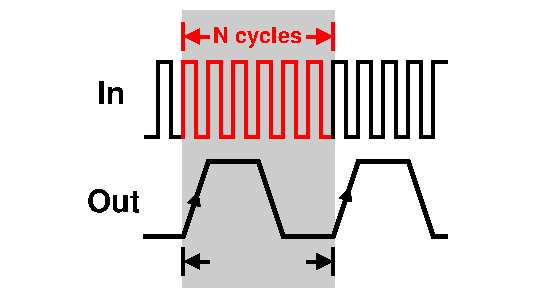
\includegraphics[scale=0.90000]{./figs/digital_div.pdf}\\
   % translate x=-16 y=516 scale 0.38
   \putbox{1.30500in}{0.16200in}{1.20}{$\mathrm{N}/f_{osc}$}%
   } % close 'parbox'
   } % close 'scalebox'
   \vspace{-\baselineskip} % this is not necessary, but looks better
\fontfamily{\rmdefault}\selectfont
